\documentclass[a4paper,11pt ]{report}
\usepackage[toc,page]{appendix}
\usepackage[T1]{fontenc}
\usepackage[utf8]{inputenc}
\usepackage[english]{babel}
\usepackage[style=numeric, maxnames=99, firstinits=true]{biblatex}
\usepackage{subfig}
\usepackage{guit}
\usepackage{titlesec} 
\usepackage{amssymb}
\usepackage{amsmath}
\usepackage{amsthm}
\usepackage{eurosym}
%\usepackage{makeidx}
\usepackage{caption}
\usepackage{tikz}
\usetikzlibrary{matrix}
\usepackage[siunitx,european]{circuitikz}
\usepackage{tikz}
\usepackage{epstopdf}
\usepackage{amsthm}

% Macro to define the norm
\usepackage{mathtools}
\DeclarePairedDelimiterX{\norm}[1]{\lVert}{\rVert}{#1}

% Macro to define the Definition environment
\theoremstyle{definition}
\newtheorem{definition}{Definition}

\bibliography{SemesterProject}


\begin{document}
%----------------------------------------------------------------------
%       TITLE PAGE
%----------------------------------------------------------------------
\begin{titlepage}
    \begin{center}
        
\includegraphics[width=0.5\textwidth]{img/logo}~\\[0.3cm]
        \textsc{\Large EPFL Semester Project -- Spring 2016}\\[0.5cm]
        \hrule
        \hspace{0.8cm}
        { \huge{ \bfseries Explicit stabilized methods for numerical integration of \textsc{Neuron}'s equations}}
        \hrule 
        \begin{minipage}{0.4\textwidth}
            \begin{flushleft} \large
                \emph{Author:}\\
                Nicol\`o \textsc{Ripamonti}\\
                Sciper n. 260853
            \end{flushleft}
        \end{minipage}
        \begin{minipage}{0.4\textwidth}
            \begin{flushright} \large
                \emph{Supervisors:} \\
                Casalegno Francesco\\
                Rosilho de Souza Giacomo\\
                \bigskip
                \emph{Responsible:} \\
                Prof. Abdulle Assyr
            \end{flushright}
        \end{minipage}
        \vfill
        {\large \today}
    \end{center}
\end{titlepage}


%----------------------------------------------------------------------
%      TABLE OF CONTENTS 
%----------------------------------------------------------------------
\tableofcontents
%\setcounter{chapter}{-1}


%----------------------------------------------------------------------
%      INTRODUCTION 
%----------------------------------------------------------------------
\chapter{Introduction}
\addcontentsline{toc}{chapter}{Introduction}


%----------------------------------------------------------------------
%       CHAPTERS
%----------------------------------------------------------------------

\chapter{Biological model}
Brief introduction ...
\section{The Hodgkin--Huxley model}
Say who introduced the model.. Talk about HH\\
Experimental results show that the process of depolarization of the surface membrane of a nerve fibre could be modeled as an equivalent electrical circuit (see Figure \ref{equiv_circuit}). 
\begin{figure}
\begin{center}
\begin{circuitikz}
	\draw [o-](0,0) node[anchor=east]{Inside}
		to (0,1.5);
	\draw [o-](0,7.5) node[anchor=east]{Outside}
		to (0,6) ;
	\draw(-1.2,1.5) 
		to (1.2,1.5)
		to [battery1, l_=$V_K$](1.2,3)
		to [american resistor, l_=$\frac{1}{g_K}$,i_<=$I_K$](1.2,6)
		to (-1.2,6)
		to [american resistor, l^=$\frac{1}{g_{Na}}$,i>^=$I_{Na}$](-1.2,3)
		to [battery1, l=$V_{Na}$](-1.2,1.5); % central box
	\draw (-1.2,1.5)
		to (-3.6,1.5)
		to [capacitor, l^=$C_M$](-3.6,6)
		to (-1.2,6); % right box
	\draw (1.2,1.5)
		to (3.6,1.5)
		to [battery1, l_=$V_l$](3.6,3)
		to [american resistor, l_=$\frac{1}{g_L}$,i_<=$I_L$](3.6,6)
		to (1.2,6); % left box 	
\end{circuitikz}
\end{center}\caption{Equivalent electrical circuit}
\end{figure}\label{equiv_circuit}
It is important to underline that Hodgkin and Huxley derived their model not by describing the molecular events related to changes in permeability but they were driven by some questions regarding the general behaviour of cellular membrane\cite{main_paper_HH}. Their starting assumption, verified later by data, was that the membrane permeability is influenced by the membrane potential and not by the membrane current: a   
direct consequence is that the main contribution to membrane permeability is the effect of electric fields on distribution of charged particles. This result shows the importance of including in the model the mechanism of the ions crossing the membrane (in particular sodium and potassium)

Unfortunately, at their time, they were only able to reject previously accepted assumptions and models but thanks to a exaustive study of nerve cells of squid giant axon, they got a more in-depth view of some properties of the membrane, like the steep relation between its potential and the ionic conductance. 

Even small changes in the potential are followed by a e-fold increase in the ionic conductances of sodium and potassium: the effect of this phenomenon is of great importance since it affects the difference in ionic concentration between the inside of the cell and the extracellular liquid which in its turn generates a Nerst's potential that can be represented by a battery in the simplified circuit. 

Another observed property is the behaviour of the membrane with respect to an imbalance between input and output current, i.e. more positive charges enter the cell than leave it or viceversa, which made them think that capacitive effects come into play to change membrane potential, which polarise or depolarise according to the change in the total charge. All these observations, combined with their previous hypothesis, were used to build a solid theoretical framework from which a set of equations could be developed.
\section{Mathematical description}
The total membrane current can be written as the sum of a capacity current (modeled as a perfect electrical capacitor without dielectric loss) and of an ionic current.
\begin{equation}\label{eq:1}
I=C_M\frac{\partial V}{\partial t}+I_i,
\end{equation}
In (\ref{eq:1}) we used the following notation:
\begin{align*}
&I \quad \text{is the total membrane current density [mA]}\\
&I_i \quad \text{is the ionic current density [mA]}\\
&V \quad \text{is the displacement of membrane potential from its resting value [mV]}\\
&C_M \quad \text{is the membrane capacity per unit area [...]}\\
&t \quad \text{is the time [...]}
\end{align*}
The choice of model the currents in parallel is due to the similarity between ionic current when $\frac{dV}{dt}=0$ and the capacity current when $I=0$. This model is enriched by identifying the different contributions for the ionic current, as follows:
\begin{equation*}
I_i=I_\text{Na}+I_\text{K}+I_\text{L},
\end{equation*}
where $I_\text{Na}$ and $I_\text{K}$ are the components related to  different ions channels (Na=Sodium, K=Potassium) and $I_\text{K}$ is the leak current. Using Ohm's law, expressed in term of conductance (i.e. $I=gV$), yields the equation, 
\begin{align*}
I_i&=g_\text{Na}(V-V_\text{Na})+g_\text{K}(V-V_\text{K})+g_\text{L}(V-V_\text{L}),
\end{align*}
where $V$,$V_\text{Na}$,$V_\text{K}$ and $V_\text{L}$ are the displacements from resting potentials. The sign of the individual ionic contribution can be positive or negative depending on the relation between the membrane voltage and the ionic potential: this can can lead to a problem of sign conventions, which is solved by setting positive a ionic current flowing out of the cell.

 As said before, the conductance of sodium and potassium channel show a strong dependence on membrane potential, while $g_\text{L}$ is usually taken as a constant: this is called leakage conductance and its value is smaller than the voltage-dependent conductances. Although Hodgkin and Huxley did not know the complex mechanism behind the rise and fall of ionic conductances, they were were able to reconstruct this relation by fitting their experimental results (see Figure (\ref{rise_fall_potassium})).\\
\begin{figure}[h!]
\centering
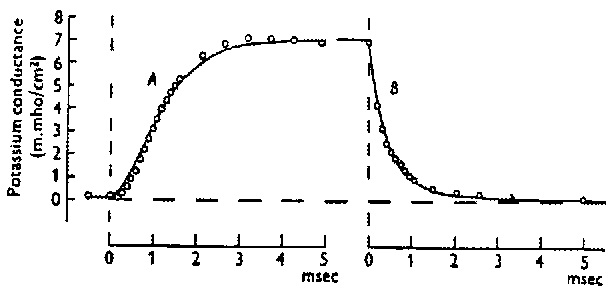
\includegraphics[scale=0.7]{rise_fall_potassium}
\caption{\small Rise and fall of potassium conductance associated with a depolarization and a polarization of $25\text{ mV}$}
\label{rise_fall_potassium}
\end{figure}

Without any first principles avalaible they observed that the potassium conductance is proportional to the fourth power of the solution of a first order equation in the following sense
\begin{align}\label{gate_n}
g_\text{K}&=\bar{g}_\text{K}n^4,\nonumber\\
\frac{dn}{dt}&=\alpha_n(1-n)-\beta_nn,
\end{align}
where $\bar{g}_\text{K}$ has the dimension of a conductance/$\text{cm}^2$, $\alpha_n$ and $\beta_n$ are constant in time but depend on membrane potential $V$ and $n$ is a dimensionless variable constrained between $0$ and $1$. In the resting state $\text{V}=0$, $n$ has the value
\begin{equation*}
n_0=\frac{\alpha_n\vert_{V=0}}{\alpha_n\vert_{V=0}+\beta_n\vert_{V=0}}.
\end{equation*}
In order to obtain an explicit formulation for $\alpha_n$ and $\beta_n$, many measuraments were taken at different temperatures, ionic concentrations and membrane potential configurations and then plotted against the resting potential $\text{V}$ to give the following result
\begin{align*}
\alpha_n&=0.01\frac{\textit{V}+10}{e^{\frac{\textit{V}+10}{10}}-1},\\
\beta_n&=0.125e^{\frac{\textit{V}}{80}},
\end{align*}
where the functions $\alpha_n$ and $\beta_n$ are measured in ms and \textit{V} is measured in mV. They noticed that during the depolarisation phase the variation in $g_\text{K}$ has a sigmmoid shape, while the polarisation phase behaves as a decaying exponential: this situations are captured very well by $\alpha_n$ and $\beta_n$ respectively. The fourth power that relates $n$ to $g_{\text{K}}$ is related to the number of first-order processes that have to occur in order to have the desired curvature of the sigmoid function: the more numerous they are, the more steep the shape will be. This is compatible with their educated guess (verified several years later) that each ionic channel contains several gates, and all of them have to be open in order to have an open channel (and so a sigmoid depolarisation) while it is sufficient that one of them is closed to shut the channel (hence the exponentially decaying polarisation). After this physical explanation, $n$ can be interpreted as the probability for a given gate to be open: if we extend this to the more realistic case of a large number of channels, it becomes the fraction of the total number of gates that are in the permessive state (N.B. The definition of permissive/non-permissive state of the gate is a little bit different from the definition of open/close and it was given later than \cite{main_paper_HH}, but still today $\alpha$ and $\beta$ represents the transition between this two states).\\
Regarding the sodium conductance, the procedure followed is only slightly different from the one adopted for the potassium. As before the idea is that the conductance is related to a certain number of first order process, but while for the potassium these processes are all of the same kind, described by the gate state $n$, now we have two different variables that come into play. This led them to the following assumptions:
\begin{align}
g_\text{Na}&=m^3h\bar{g}_\text{Na},\nonumber\\
\frac{dm}{dt}&=\alpha_m(1-m)-\beta_mm,\label{gate_m}\\
\frac{dh}{dt}&=\alpha_h(1-h)-\beta_hh\label{gate_h},
\end{align}
where $\bar{g}_\text{Na}$ is a constant and the $\alpha$'s and $\beta$'s depend on V but not on time. Here $h$ plays an opposite role of what $n$ did for the potassium channels: in this case we consider it to be means when the channel is inactive and we have the polarisation phase. On the other hand, $m$ behaves as $n$, with the only difference that for sodium ion channels the steepness of the relation between gate conductance and membrane potential is given by only $3$ of these gates instead of $4$ as before. However, even if all these \enquote{activating} gates $m$ are open, but the \enquote{inactivating} gate $h$ is open, then the channel remains closed. The initial states for the first-order equations describing the transition rates are again
\begin{align*}
m_0&=\frac{\alpha_m\vert_{V_0}}{\alpha_m\vert_{V_0}+\beta_m\vert_{V_0}},\\
h_0&=\frac{\alpha_h\vert_{V_0}}{\alpha_h\vert_{V_0}+\beta_h\vert_{V_0}}.
\end{align*}
Now that we have all the coefficients, we can rewrite (\ref{eq:1}) as
\begin{equation}\label{demifinal}
I=C_M\frac{\partial V}{\partial t}+\bar{g}_\text{K}n^4(V-V_\text{K})+ \bar{g}_\text{Na}m^3h(V-V_\text{Na})+\bar{g}_\text{L}(V-V_\text{L}).
\end{equation}
For the cable approximation of the axon, which is surrounded by a large amount of conducting fluid, the membrane current, in the case of a propagated action potential, is related to the potential $V$ by the following electrostatical relation
\begin{equation*}
I=\frac{1}{2aR}\frac{\partial}{\partial x}\left(a^2\frac{\partial V}{\partial x}\right),
\end{equation*} 
where $R$ is the cytoplasmatic resistivity and $a$ the axon radius, which may vary along the cable.
Hence, after rearranging equation (\ref{demifinal}) to take into account the unit of measuraments used for the experimental setting, we obtain
\begin{align}\label{final}
10^{-3}C_M\frac{\partial V}{\partial t}=&\frac{10^4}{2aR}\frac{\partial}{\partial x}\left(a^2\frac{\partial V}{\partial x}\right) \nonumber\\
&-\bar{g}_\text{K}n^4(V-V_\text{K})- \bar{g}_\text{Na}m^3h(V-V_\text{Na})-\bar{g}_\text{L}(V-V_\text{L})\\
&-\frac{10^2g_{syn}y}{2\pi a}\delta_{syn}(x)(V-V_{syn}) \nonumber,
\end{align}
in which the most simple modelization of synaptic interaction is considered ($g_{syn}(y)$), depending only on the synaptic receptor state $y$ evolving as
\begin{equation*}
y(t)=\frac{t-t_{\mathrm{off}}}{\tau}e^{\left(-\frac{t-t_{\mathrm{off}}-\tau}{\tau}\right)}
\end{equation*}
This is a simple, yet effective, description of an incoming spike in the potential, able to capture the nature of the synaptic behaviour, but also to allow fast and efficient computation, required in the case of large neural networks.
\section{Domain and boundary conditions}
The model described in the previous section is applied on a domain which can be schematized on a domain as the one represented in Figure (\ref{fig:hines_branch}).
\begin{figure}[h!]
\centering
\subfloat{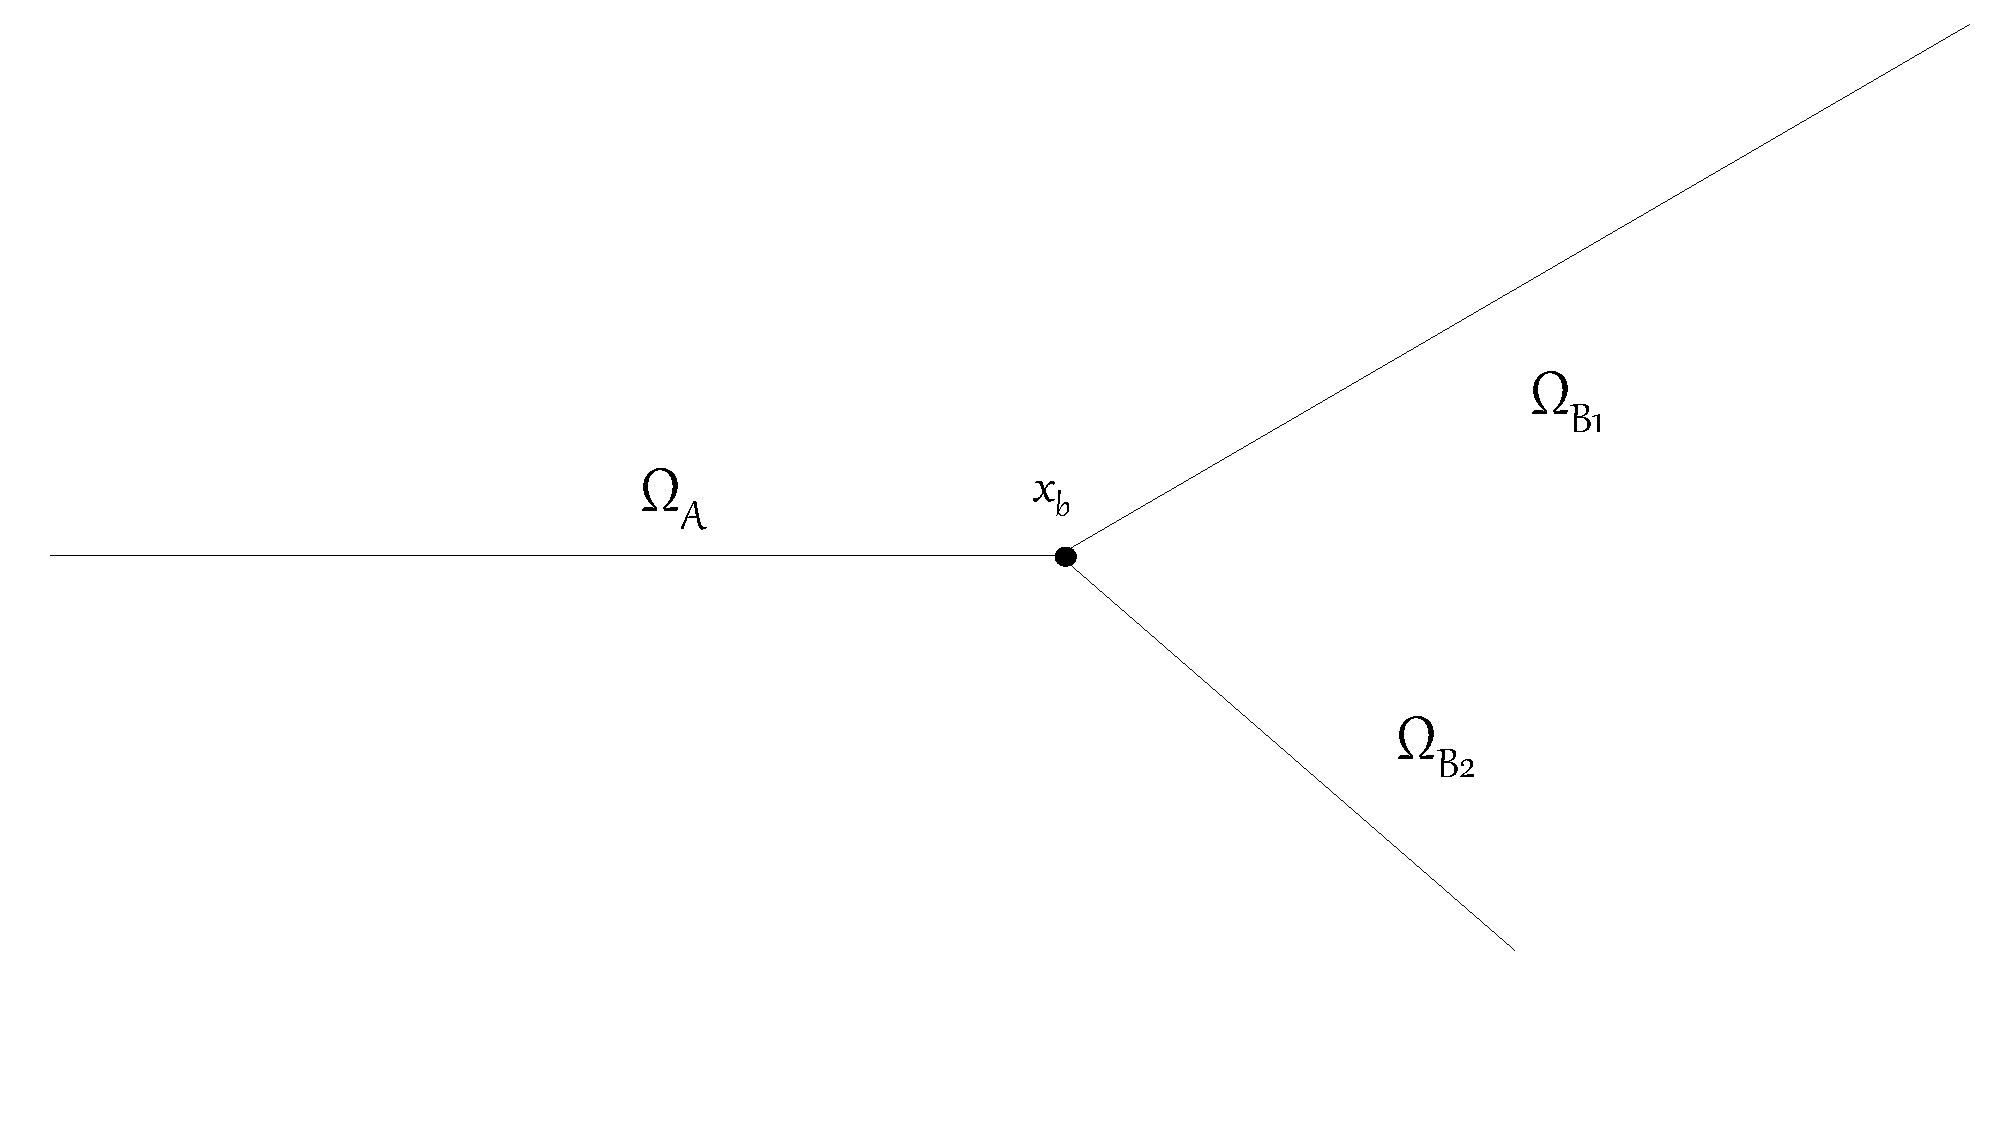
\includegraphics[scale=0.37]{hines_scheme.pdf}}
\caption{Dendritic tree with one branching node.}
\label{fig:hines_branch}
\end{figure}
The unbranched sections of the neuron are represented as $1$D segments, an approximation due to the difference between length and thickness of each branch: this entails that all the variables considered are function of the axial abscissa along the cable but not of the radial distance from the center. This model is acceptable if the real radius, even if variable, show only relative deviations with respect to its mean value: some problem may occur if, for instance, we consider a tapered dendrite.\\
To set the boundary conditions and then complete the statement of the problem, electrostatic consideration are needed: the current between two points $x$ and $x+\Delta x$ is proportional to the voltage difference and the inverse of membrane resistance, thus
\begin{equation*}
I(x)=\frac{\pi a^2}{R}\frac{V(x-\Delta x)-V(x)}{\Delta x},
\end{equation*}
and by taking the limit $\Delta x \rightarrow 0$ we have
\begin{equation*}
I(x)=\frac{\pi a^2}{R}\frac{\partial V}{\partial x}.
\end{equation*}
In the branching node, Kirchoff's law for the conservation of electric charge that 
\begin{equation*}
\left( a^2\frac{\partial V}{\partial x}\right)\bigg|_{x=x_b}^A-\left( a^2\frac{\partial V}{\partial x}\right)\bigg|_{x=x_b}^{B_1}-\left( a^2\frac{\partial V}{\partial x}\right)\bigg|_{x=x_b}^{B_2}=0,
\end{equation*}
which is chosen as boundary condition in the branching node $x_b$.\\
On the terminal points it is assumed that no current flows outside or inside, giving homogeneous Neumann conditions
\begin{equation*}
\frac{\partial V}{\partial x}=0.
\end{equation*}

\chapter{Spatial discretization}
\section{Finite differences}
The partial differential equations (PDEs) (\ref{final}),(\ref{gate_n}),(\ref{gate_m}) and (\ref{gate_h}) are replaced by a system of ordinary differential equations (ODEs), using a technique known as \emph{method of lines}. The idea is to discretize all the dimensions of the problem but one (time in our case) and then solving the resulting equation (ODEs). First we need to define a mesh: on the internal regions of the dendrite a uniform mesh with spacing $h$ is used, while for the elements near the boundary for which is reduced to $\frac{h}{2}$ (TODO: spiega perchè è più fine sul bordo, motivi di convergenza e chiedi a Francesco il motivo bio).\\
\begin{figure}[h!]
\centering
\subfloat{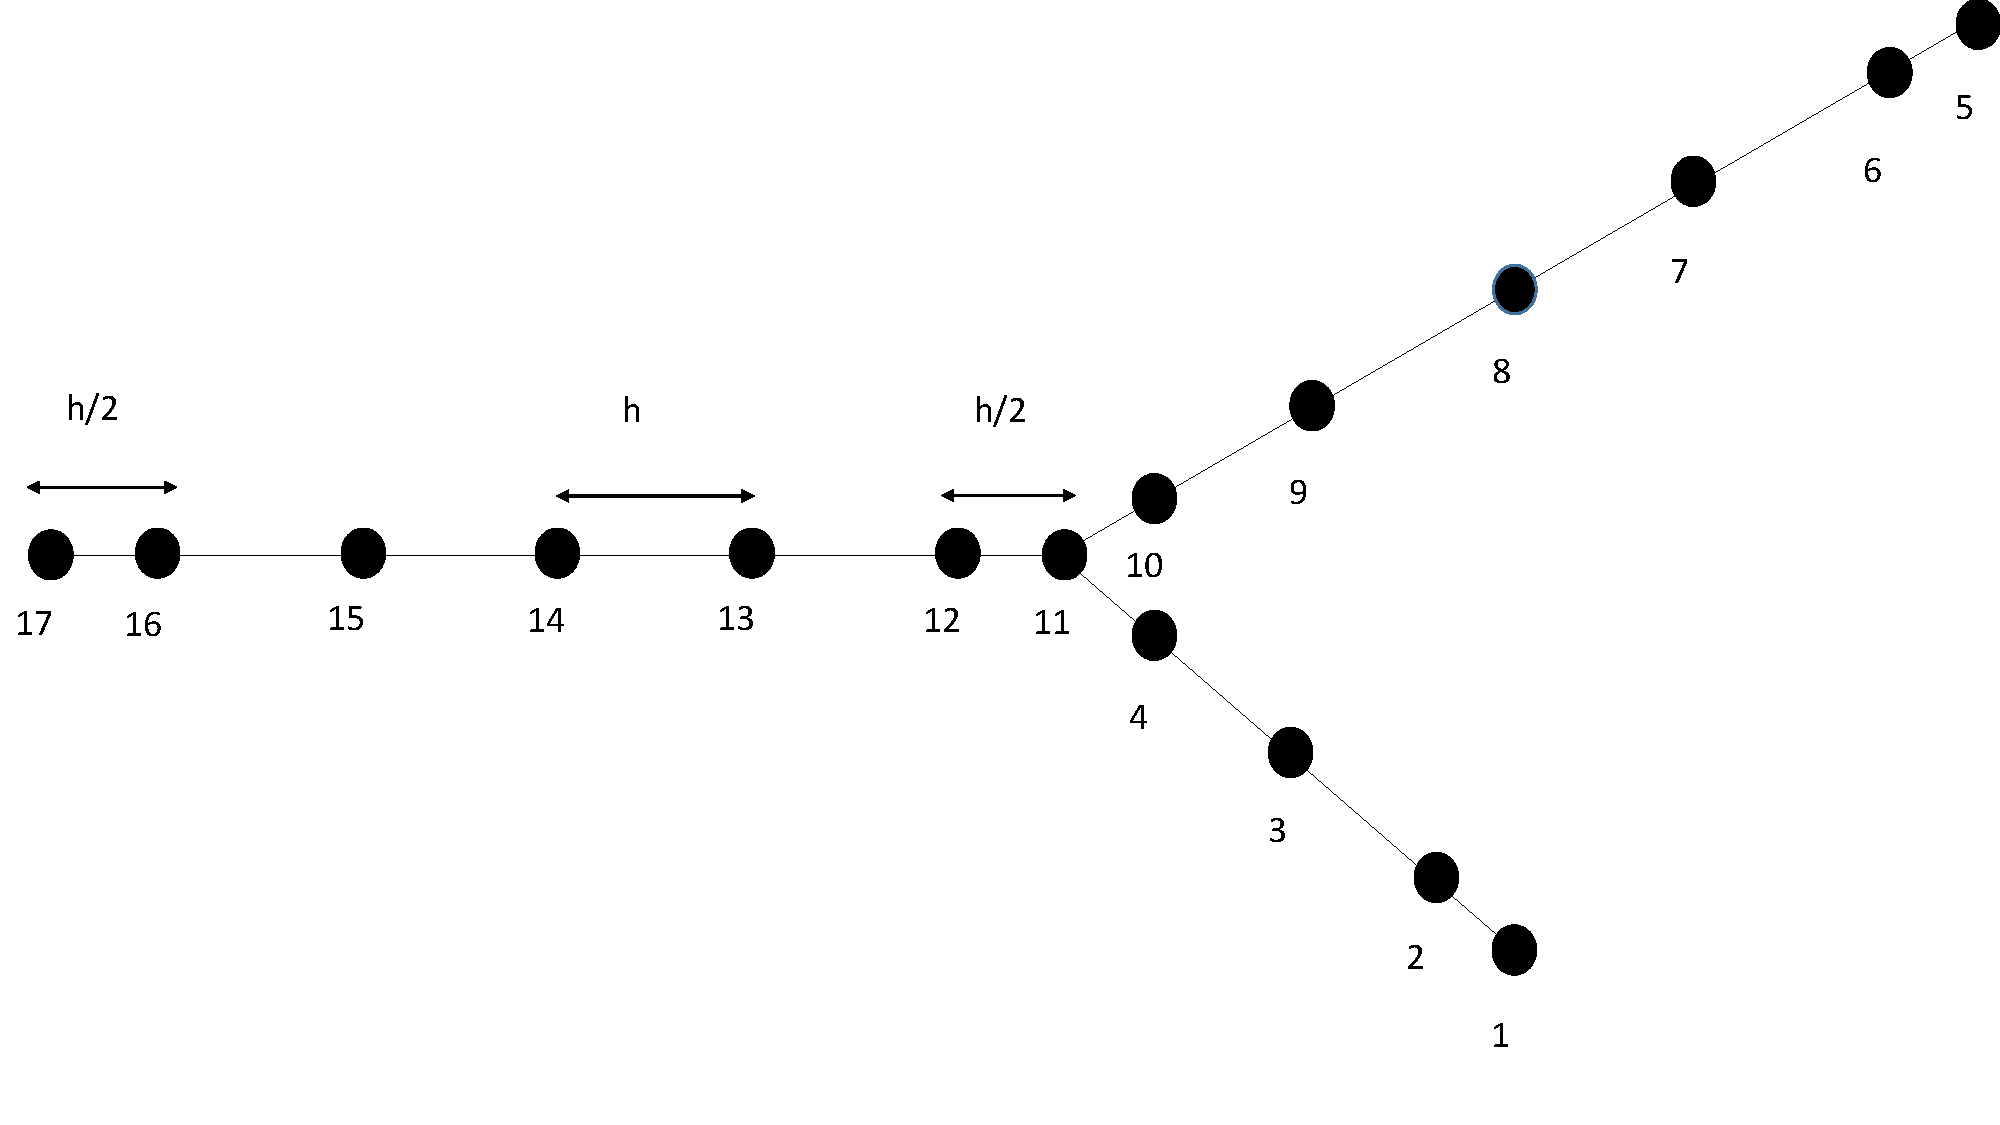
\includegraphics[scale=0.37]{hines.pdf}}
\caption{Example of mesh used }
\end{figure} 

A possible starting point for the discretization is to look at finite differences centered at each point $x_j$ of the mesh: for the points far from boundaries the following standard results for uniform grid can be used
\begin{equation*}
\frac{\partial f}{\partial x}=\frac{f(x+\frac{\Delta x}{2})-f(x-\frac{\Delta x}{2})}{\Delta x}+\mathcal{O}((\Delta x)^2),
\end{equation*}
which is a second order centered approximation of the first order derivative of a function. By applying this form twice in the d\printbibliography
iffusive term of (\ref{final}) we get to 
\begin{equation*}
\frac{\partial}{\partial x}\left( a^2 \frac{\partial V}{\partial x}\right)\approx a^2\frac{V(x+\Delta x)-2V(x)+V(x-\Delta x)}{(\Delta x)^2},
\end{equation*}
in the case of $a$ constant.\\
Near the terminal and ending nodes the situation is more subtle because of the nonuniformity of the grid and so we need to go more in depth with Taylor series: we report, as example, the case of the last node of the branch $\Omega_A$.\\ 
\begin{figure}[h!]
\centering
\subfloat{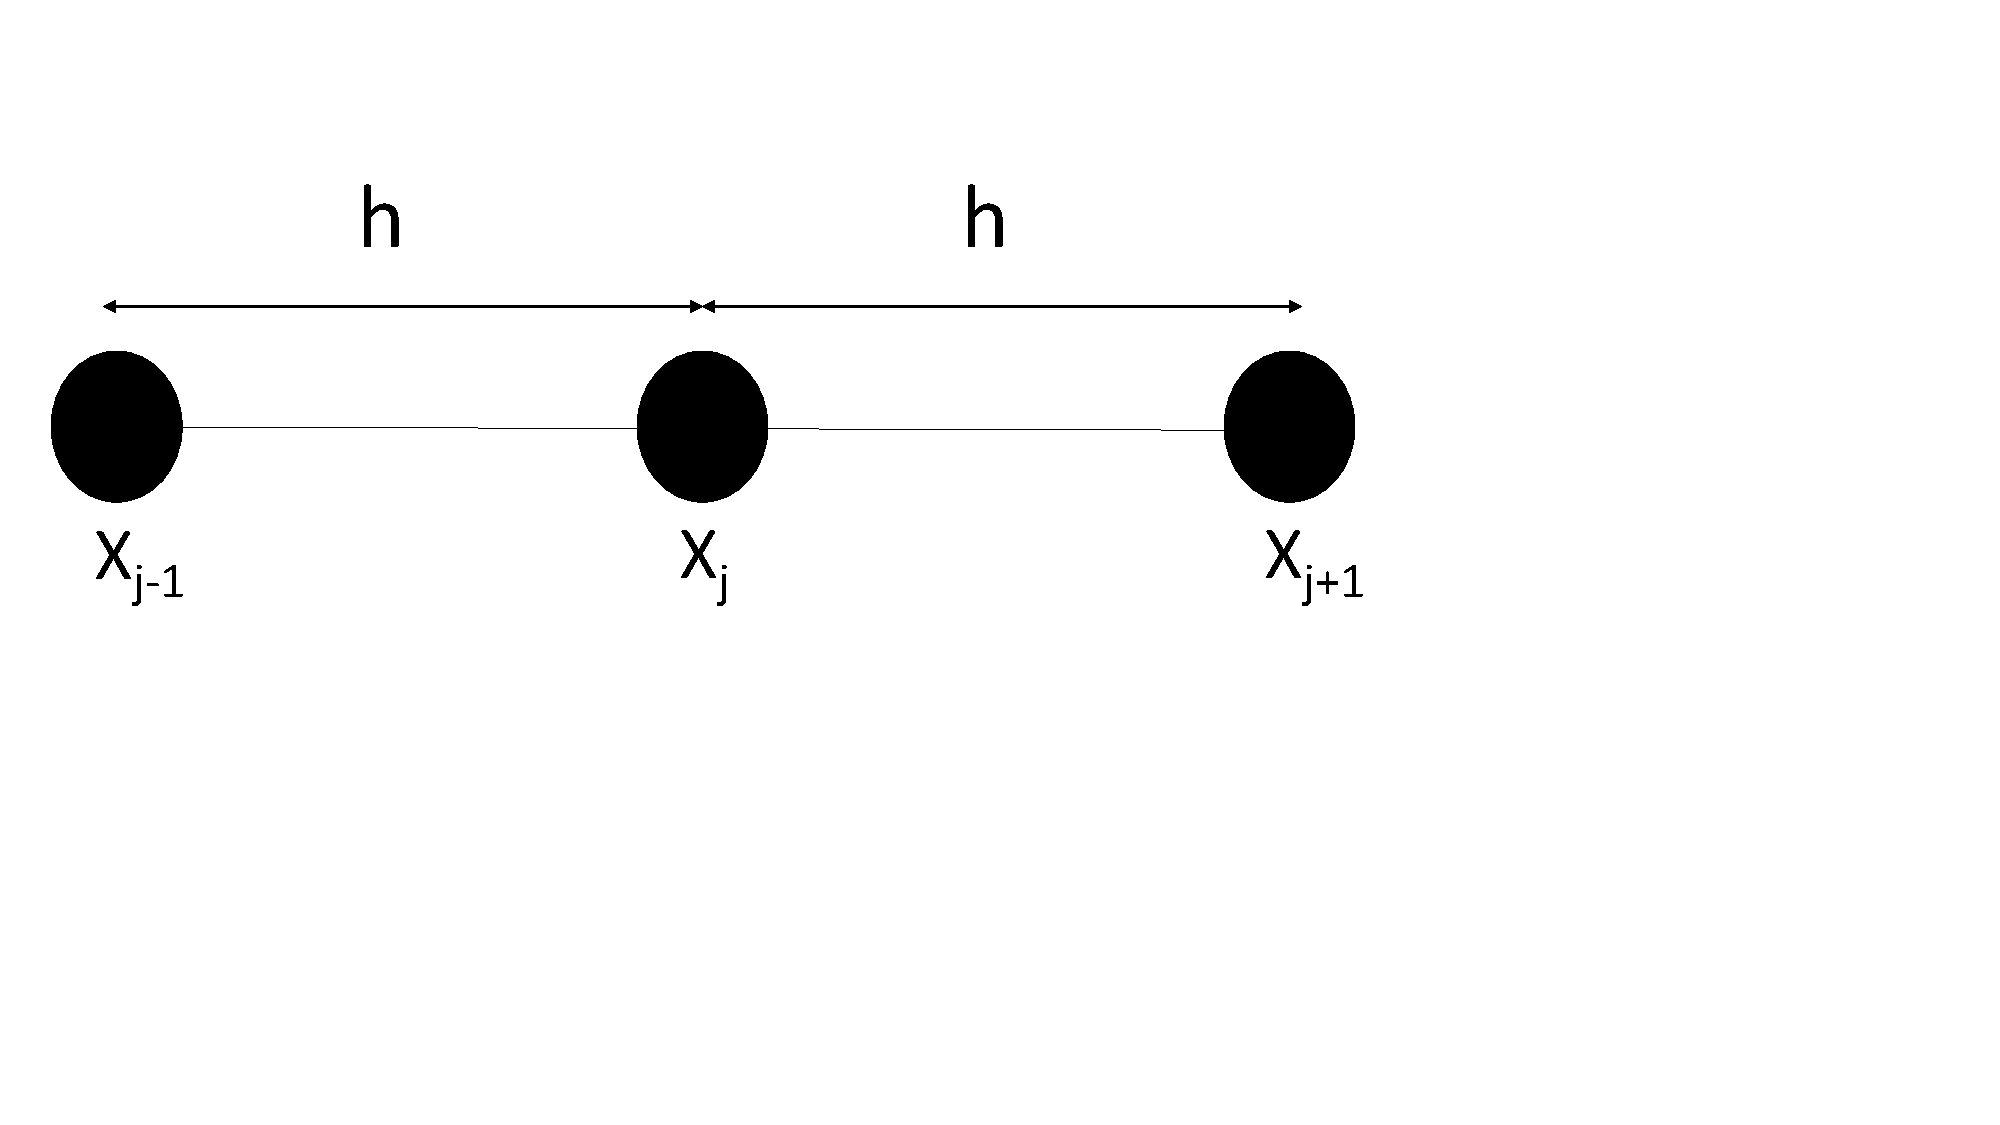
\includegraphics[scale=0.2]{hines_uniform_branch.pdf}}
\subfloat{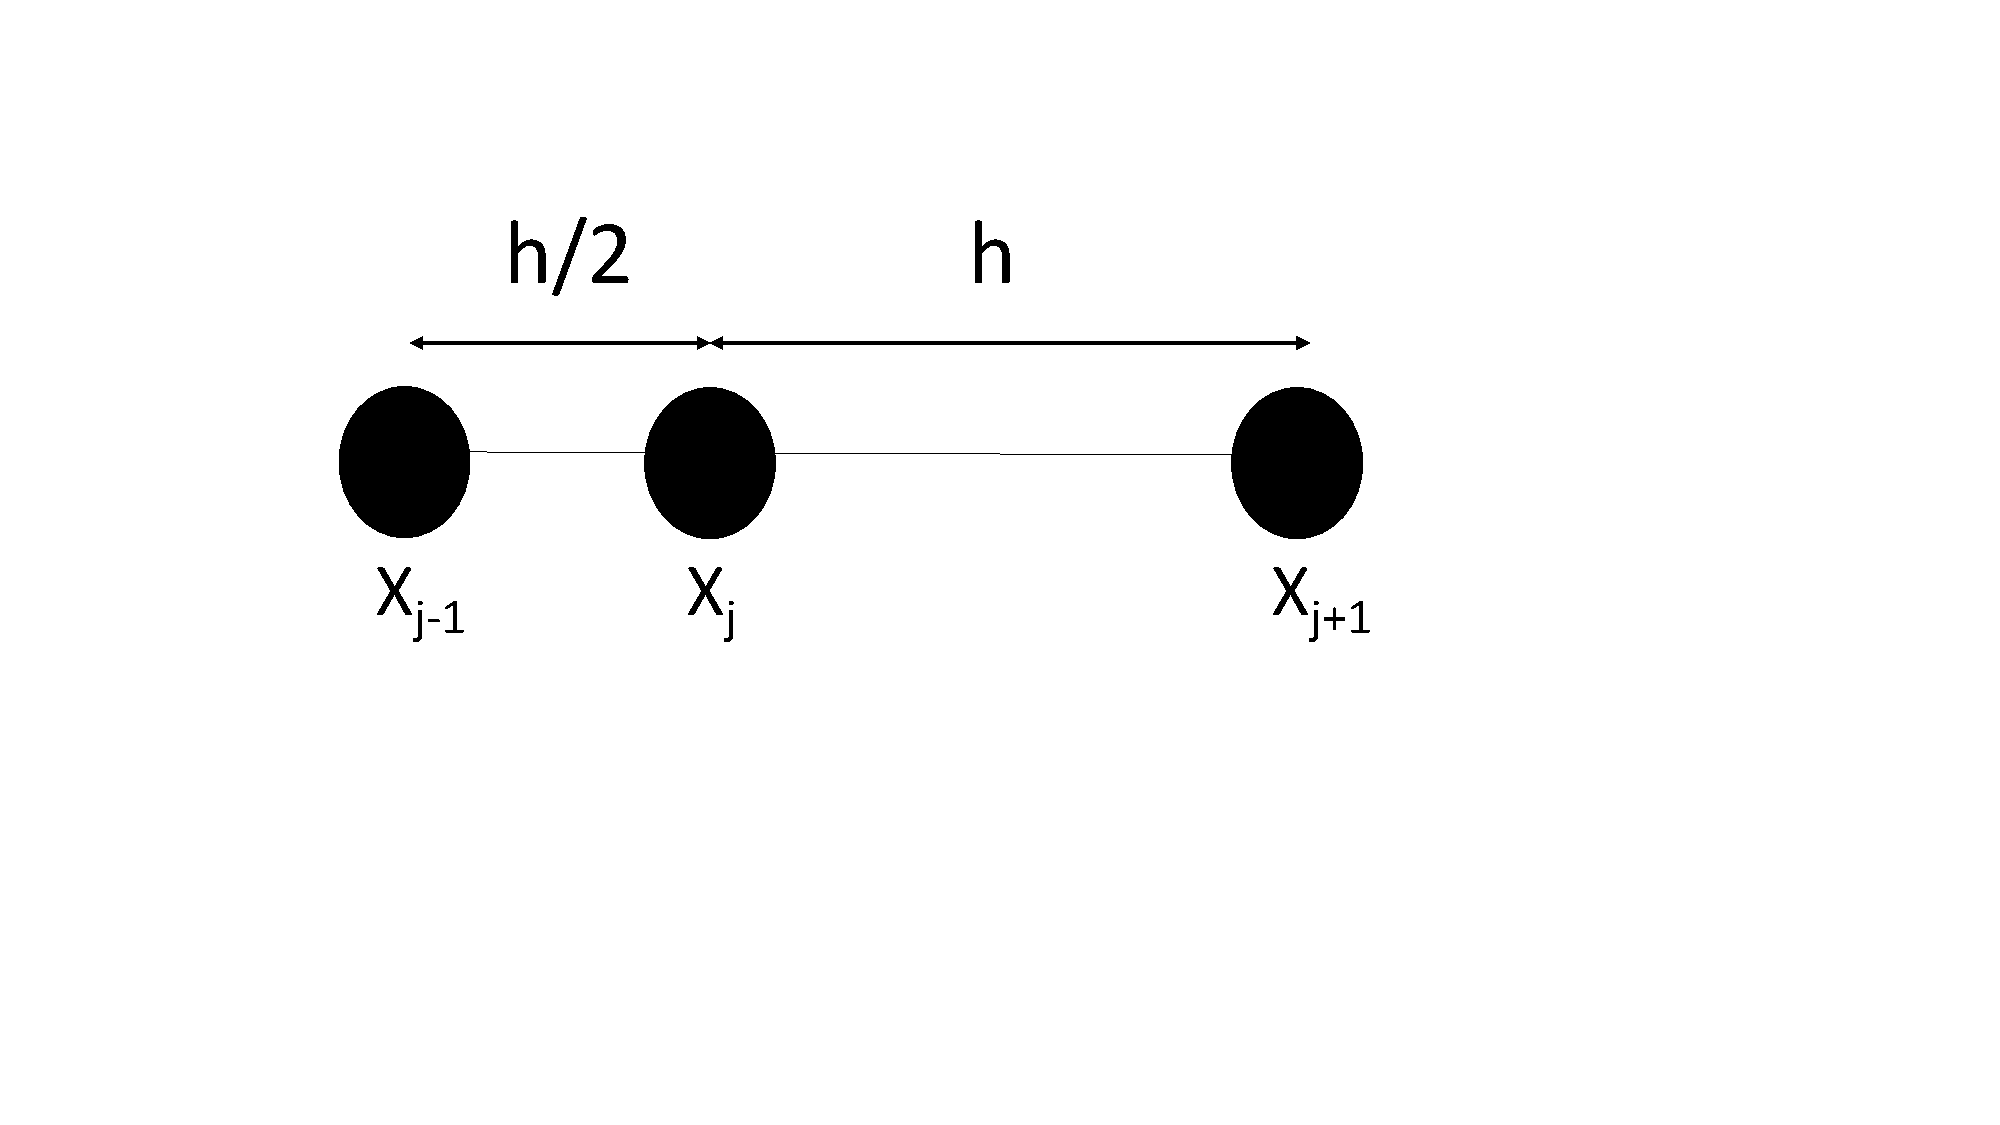
\includegraphics[scale=0.2]{hines_non_uniform_branch.pdf}}
\caption{Local region in the middle of the mesh (left) and near the terminal point of the branch $\Omega_A$ (right)}
\end{figure}

Consider 
\begin{align*}
f(x_{j+\frac{1}{2}})&=f(x_j)+\frac{\partial f}{\partial x}(x)\bigg|_{x=x_j}\frac{\Delta x}{2}+\frac{\partial^2 f}{\partial x^2}(x)\bigg|_{x=x_j}\left( \frac{\Delta x}{2}\right)^2+\mathcal{O}((\Delta x)^3),\\
f(x_{j-\frac{1}{2}})&=f(x_j)-\frac{\partial f}{\partial x}(x)\bigg|_{x=x_j}\frac{\Delta x}{4}+\frac{\partial^2 f}{\partial x^2}(x)\bigg|_{x=x_j}\left( \frac{\Delta x}{4}\right)^2+\mathcal{O}((\Delta x)^3),
\end{align*}
and by combining them you get
\begin{equation*}
\frac{\partial f}{\partial x}(x)\bigg|_{x=x_j}=\frac{f(x_{j+\frac{1}{2}})+3f(x_j)-4f(x_{j-\frac{1}{2}})}{\frac{3}{2}\Delta x}+\mathcal{O}((\Delta x)^2)
\end{equation*}



\section{Node enumeration}

\chapter{Time integration}

\section{Stability of numerical integrators}

\subsection{Examples}

\subsection{Linear stability analysis}
The more general case we can face is the non-linear non-automous ODEs
\begin{equation}
\begin{cases}
\frac{\text{d}}{\text{d} t}\textbf{y}=\textbf{f}(t,\textbf{y}), \qquad \textbf{y}\in\mathbb{R}^n, t\in[t_{1},t_{2}]\\
\textbf{y}(t_0)=\textbf{y}_0.
\end{cases}
\label{eqn:general_ODE}
\end{equation}
To study its stability behaviour we need to approximate this form to a case which is more manageable, by means of Taylor's series applied to the force term in (\ref{eqn:general_ODE}). Suppose we have a smooth solution $\boldsymbol{\phi} (t)$, we obtain
\begin{equation}
\frac{\text{d}}{\text{d} t}\textbf{y}=\textbf{f}(t,\boldsymbol{\phi}(t))+\frac{\partial \textbf{f}}{\partial \textbf{y}}(t,\boldsymbol{\phi}(t))(\textbf{y}(t)-\boldsymbol{\phi}(t))+\dots,
\label{eqn:Taylor_force}
\end{equation}
and then, by discarding all the terms of order bigger than 1 and setting $\textbf{w}(t)=\textbf{y}(t)-\boldsymbol{\phi}(t)$ in (\ref{eqn:Taylor_force}), we remain with
\begin{equation}
\frac{\text{d}}{\text{d} t}\textbf{w}=\textbf{A}(t)\textbf{w}(t),\label{eqn:after_linearization}
\end{equation}
where $\textbf{A}(t)=\frac{\partial \textbf{f}}{\partial \textbf{y}}(t,\boldsymbol{\phi}(t))$. Now we have to kill the time dependency in $\textbf{A}(t)$, by freezing $t=t_0$, in order to obtain a constant matrix $\textbf{A}_0$. By doing this, the following analysis will be valid only near the starting time and to extend it further we have to change the istant in which the time is frozen. 
For the sake of clarity now we suppose the matrix $A_0$ to be  fully diagonalizable, i.e. there exists an orthogonal matrix $\textbf{P}$ s.t.
\begin{equation}
\textbf{P}^{-1}\textbf{A}_0\textbf{P}=\textbf{D}, \qquad 
D=
  \begin{bmatrix}
    \lambda_1 &&&\\
    & \lambda_2 &&\\
    && \ddots &\\ 
    &&& \lambda_n
  \end{bmatrix}.
\label{eqn:diagonalization}
\end{equation}
This is not always the case, but even in more complex scenarios where the diagonalization is not possible, the stability can be investigated requiring different conditions to $A$. Using (\ref{eqn:diagonalization}) in (\ref{eqn:after_linearization}) we are left with a set of $n$ decoupled equations 
\begin{equation}
\frac{\text{d}}{\text{d} t}v_i=\lambda_i v_i, \qquad i=1\dots n,
\label{eqn:diagonalized_form}
\end{equation}
where $\lambda_i$-s are the eigenvalues of $A_0$. 
Each of them represents an example of Dalqhuist test equation
\begin{equation}
\frac{\text{d}}{\text{d} t}y=\lambda y, \qquad \lambda \in \mathbb{C}.
\end{equation}
The solution for this famous problem is an exponential which slope depends on the sign of $\lambda$ (Figure \ref{fig:Dahlquist}).
Hence, the meaning of (\ref{eqn:diagonalized_form}) is that even if only one of the eigenvalues of the linearized system has a real part greater than zero, then the solution is unstable \cite{Dahlquist}.
\begin{figure}
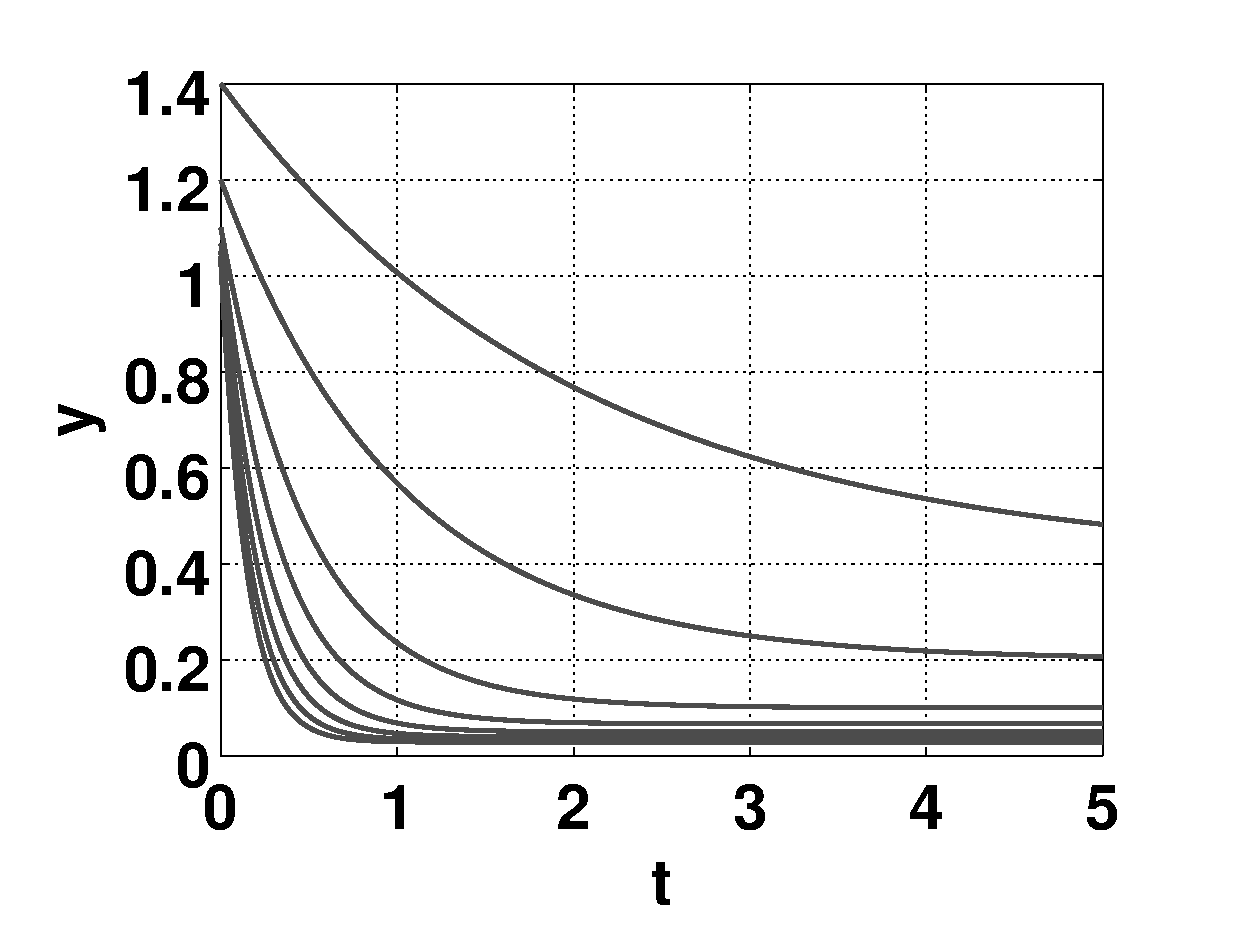
\includegraphics[width=4.15cm]{img/stable.eps}
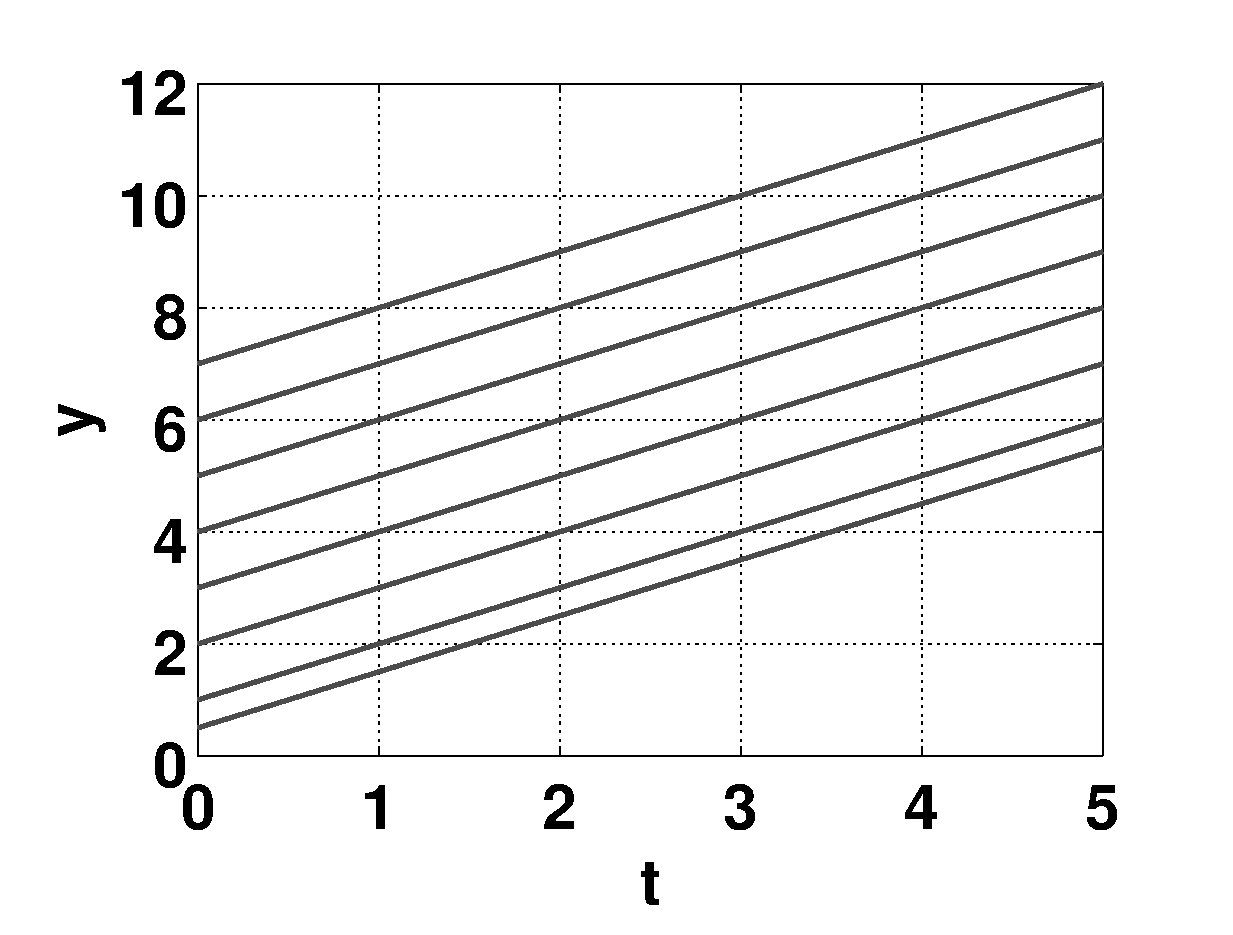
\includegraphics[width=4.15cm]{img/asyn_stable.eps}
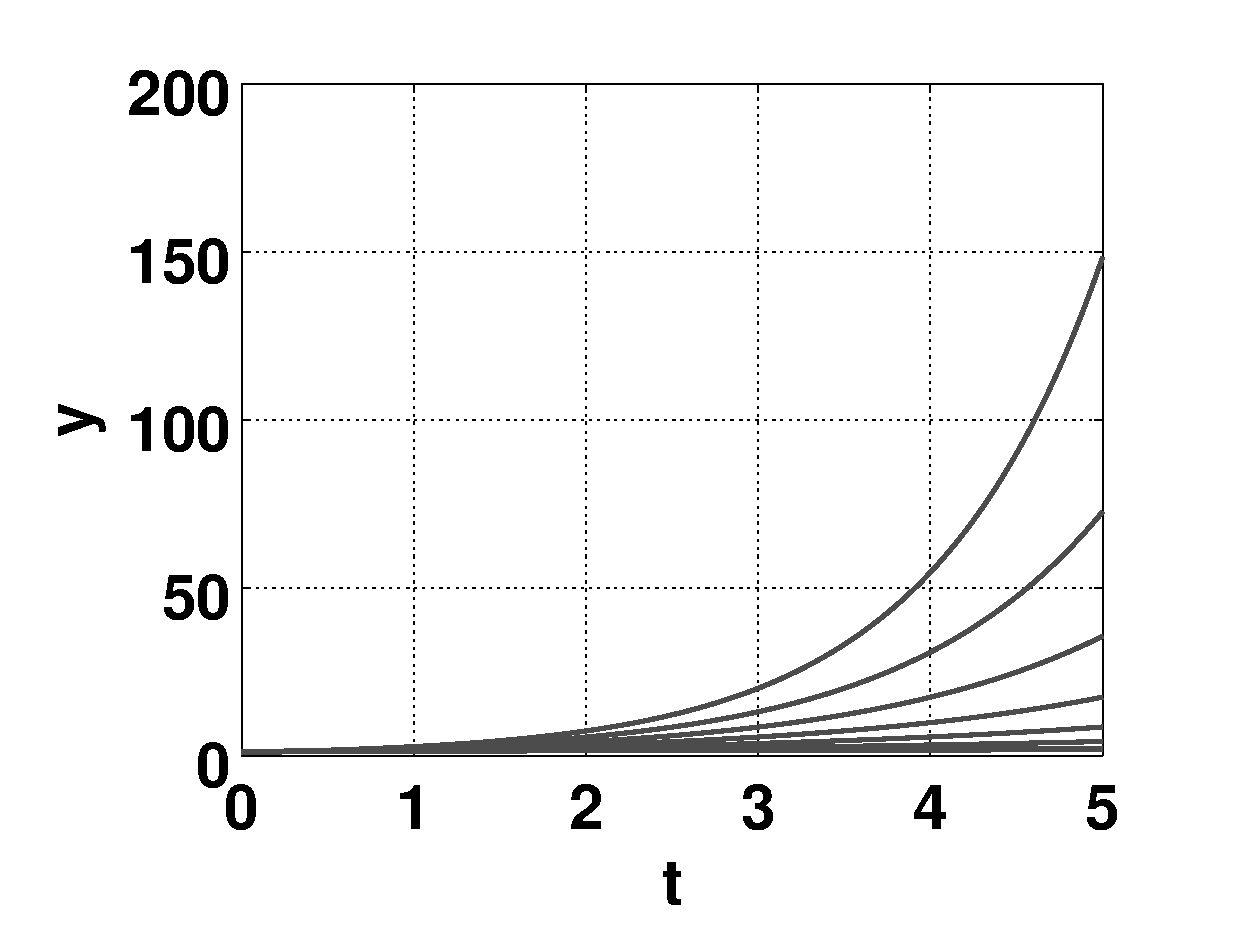
\includegraphics[width=4.15cm]{img/unstable.eps}
\caption{Solution of Dahlquist's equation for Re($\lambda$)$<0$ (stable), Re($\lambda$)$=0$ (asymptotically stable) and Re($\lambda$)$>0$ (unstable)}
\label{fig:Dahlquist}
\end{figure}
A possible definition of stability was given by Lyapunov in \cite{Lyapunov}
\theoremstyle{definition}
\begin{definition}{}
A solution to (\ref{eqn:general_ODE}) that exists for all $t\geq t_0$ is said to be stable (asyntotically stable) in the sense of Lyapunov if $\forall \epsilon>0$ $\exists \delta >0$ s.t. if $\norm{\Delta \textbf{y}} < \delta$ then
\begin{equation*}
\left( \lim_{t=\infty} \right) \quad \norm{\textbf{y}(t,t_0,\textbf{y}_0)-\textbf{y}(t,t_0,\textbf{y}_0+\Delta \textbf{y})}<\epsilon.
\end{equation*}
\end{definition}

\subsection{Stability of Runge--Kutta methods}
The Runge--Kutta (RK) methods are the most common way to solve an ODE: they are a family of explicit and implicit iterative numerical schemes. Another important group of ODEs solver is the Linear multistep methods \cite{Hairer_1}, which we will not deal with in this report. 
RK methods are based on the idea of computing the numerical solution after a time step $\Delta t$ through a weighted sum of intermediate steps, which approximate the slope of the solution at specific points $\in [t,t+\Delta t]$. Any Runge Kutta method can be presented in the following general form
\theoremstyle{definition}
\begin{definition}{}
Let $s\in\mathbb{N}^+$ and let $\text{b}_i$, $\text{a}_{ij}$ and $\text{c}_i$, $1\leq i,j \leq s$ be real numbers. A s-stage Runge-Kutta method for the integration of 
\begin{equation}
\begin{cases}
\frac{\text{d}}{\text{d} t}y=f(t,y),\\ y(t_0)=y_0,
\label{eqn:ODE_RK}
\end{cases}
\end{equation}
is given by 
\begin{align*}
\text{K}_i&=f\left( t_0+\text{c}_i\Delta t, y_0+\Delta t \sum_{j=1}^s\text{a}_{ij}\text{K}_j\right),\\
y_1&=y_0+\Delta t \sum_{i=1}^s\text{b}_i\text{K}_i.
\end{align*}
\label{def:RK_def}
\end{definition}
A RK method applied to (\ref{eqn:ODE_RK}) gives approximations at different times $\{ y_n(\Delta t, \lambda)\}_{n \geq 0}$. Also for the numerical solution is possible to define a stability domain based on bounded values.
\theoremstyle{definition}
\begin{definition}{}
The stability domain of a RK method is
\begin{equation*}
S_n = \{ z=\Delta t \lambda \in \mathbb{C} : \{ y_n(\Delta t, \lambda) \}_{n \geq 0} \quad \text{remains bounded} \}
\end{equation*}
\end{definition}
Usually this definition is reinterpreted in terms of stability function, which is introduced in the following statement
\theoremstyle{definition}
\begin{definition}{}
Following the same notation of Definition \ref{def:RK_def}, using a RK method to solve Dahlquist's test problem, we obtain after one step $y_1 = R(\Delta t \lambda)y_0$, where
\begin{align*}
R(z)&=1+\textbf{b}^{T}z(I-z\mathbb{A})^{-1}\mathbb{I}, \qquad z=\Delta t \lambda\\
\textbf{b}&=
\begin{pmatrix}
\text{b}_1\\
\vdots \\
\vdots \\
\text{b}_s
\end{pmatrix},
\quad \mathbb{A}=
\begin{pmatrix}
\text{a}_{1,1} & \text{a}_{1,2} & \hdots & \\
\text{a}_{2,1} & \ddots & & \vdots\\
&& \ddots & \text{a}_{n-1,n}\\
& \hdots & \text{a}_{n,n-1}& \text{a}_{n,n}
\end{pmatrix}
\quad
\mathbb{I}=
\begin{pmatrix}
1\\
\vdots\\
\vdots\\
1
\end{pmatrix}
\end{align*}\label{Stab_func}
is called stability function.
\label{def:stab_func}
\end{definition}{}
This function does not identify a scheme, since two different numerical methods can have the same stability function.
Since we want our method to be stable, the solution of the test problem need to be analyzed. Using Definition \ref{Stab_func} we have 
\begin{equation*}
y_n = R(\Delta t \lambda)y_{n-1} = \dots = (R(\Delta t \lambda))^n y_{0}<\infty
\end{equation*}
for every $y_{0}$ if and only if $\vert R(\Delta t \lambda) \vert < 1$, which is an equivalent characterization of the stability domain.

\begin{figure}
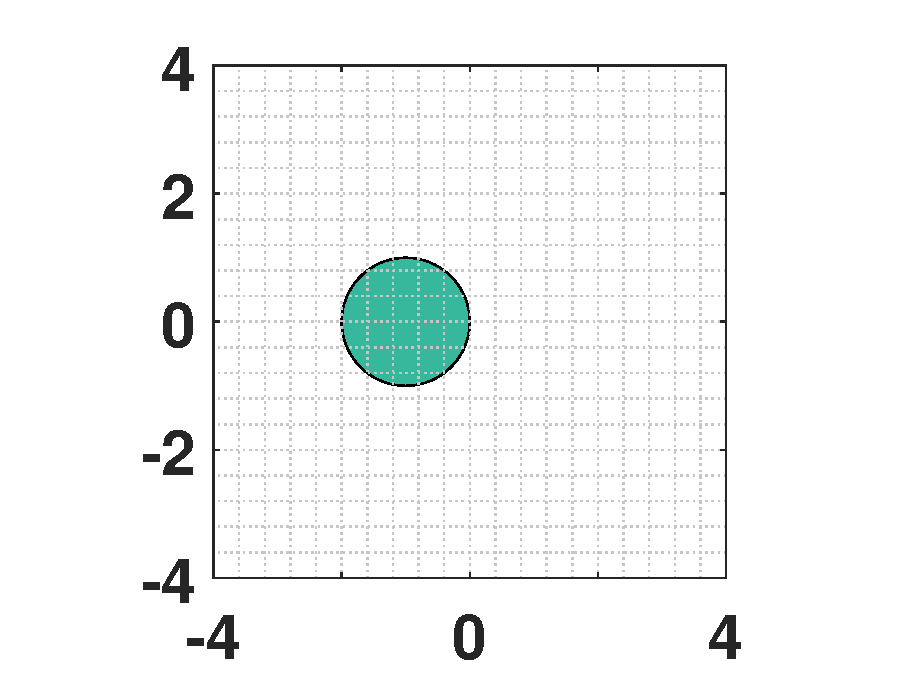
\includegraphics[width=4.15cm]{img/EE.eps}
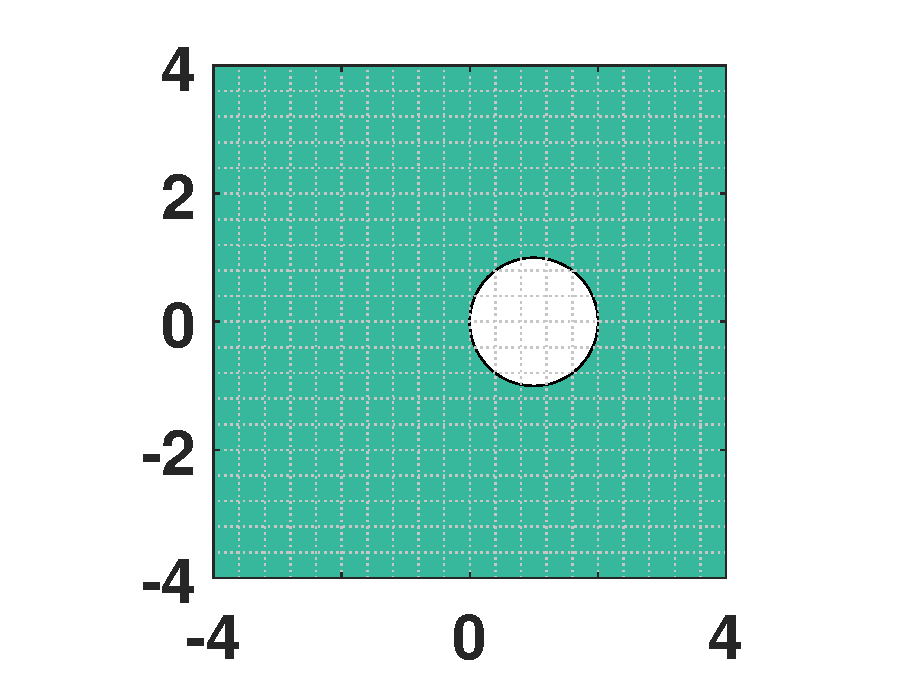
\includegraphics[width=4.15cm]{img/EI.eps}
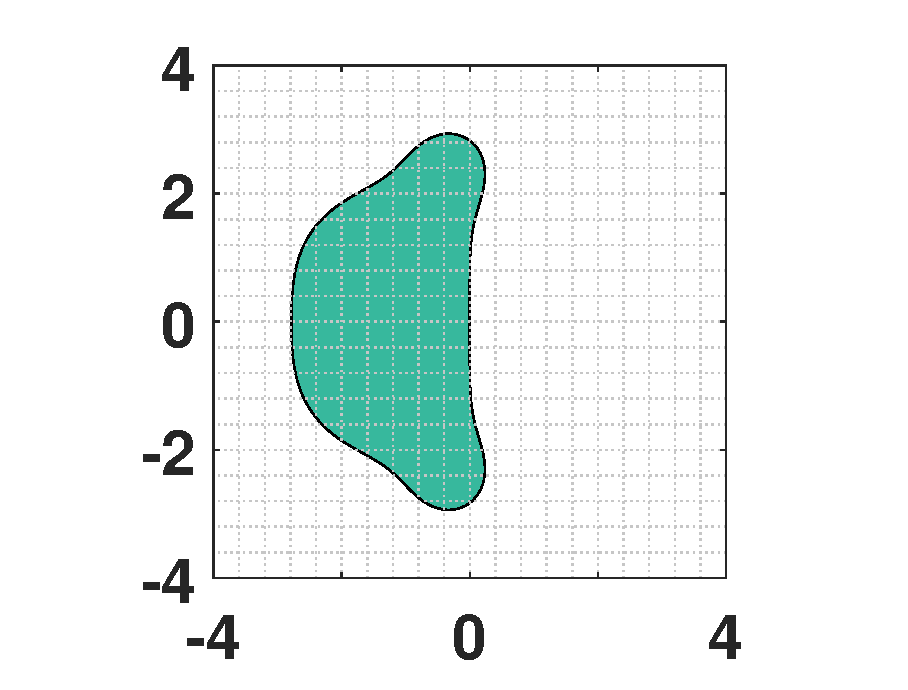
\includegraphics[width=4.15cm]{img/RK4.eps}
\caption{Stability regions of explicit Euler, implicit Euler and classical Runge-Kutta }
\end{figure}
As we have seen before, the test equation has a stable solution only if $\lambda \in \mathbb{C}^{-}$. A good property is that the numerical methods conserve the stability in the same case.
\theoremstyle{definition}
\begin{definition}{(Dahlquist 1963)}
A method, whose stability domain satisfies $S_n \in \mathbb{C}^{-}$ is called \textit{A-stable}.
\end{definition}
The stability function of a RK method can be expressed as the ratio between two polynomials of degree $\leq s$ for the implicit case and as a polynomial of the degree $\leq s$ for explicit method. Hence, by using the maximum principle theorem, it is possible to give sufficient and necessary conditions for the \text{A-stability} of a scheme.
\theoremstyle{definition}
\begin{definition}{}
A RK method is \text{A-stable} if and only if its stability function satisfies:
\begin{itemize}
\item $\vert\text{R}(iy)\vert \leq 1 \quad \forall y\in \mathbb{R}$ (also called \textit{I-stability} condition)
\item $\text{R}(z)$ is analitic in $\mathbb{C}^{-}$
\end{itemize}
\end{definition}{}
The \textit{A-stability} property ensures that our numerical solution does not explode, but there still could be some bounded oscillations. A stronger requirement is sufficient to guarante a better qualitative representation of the exact solution.
\theoremstyle{definition}
\begin{definition}{}
A RK method is \textit{L-stable} if it is \textit{A-stable} and $\lim_{z\to\infty}\text{R}(z)=0$
\end{definition}{}
The limit for $z\to\infty$ can be replaced by $z\to-\infty$, since we are dealing with rational function, so we can focus on $\mathbb{C}^-$. 

As can be seen in Figure \ref{fig:A_stability}, an \textit{L-stable} implicit method could behave better than an only \textit{A-stable} implicit method like the implicit midpoint, even if the former has a lower order of accuracy than the latter. This is due to the additional property $\text{R}(\Delta t \lambda)\approx 0$ when we have big time steps ($\Delta t \gg \lambda^{-1}$).
Since we are working with rational functions
\begin{equation}
\lim_{z\to -\infty}R(z)=\lim_{z=iy,y\to\infty}R(z),
\label{eqn:rat_func}
\end{equation}
If the stability domain of the numerical method contains only $\mathbb{C}^-$ then $\vert R(iy)\vert =1$ $\forall y\in\mathbb{R}$. But from (\ref{eqn:rat_func}) we have that, in case of $z$ with a large negative part, $R(z)$ is almost equal to 1 (but smaller). Considering the role of $R(z)$ in Definition \ref{def:stab_func}, the obscillations are only slghtly damped.
\begin{figure}
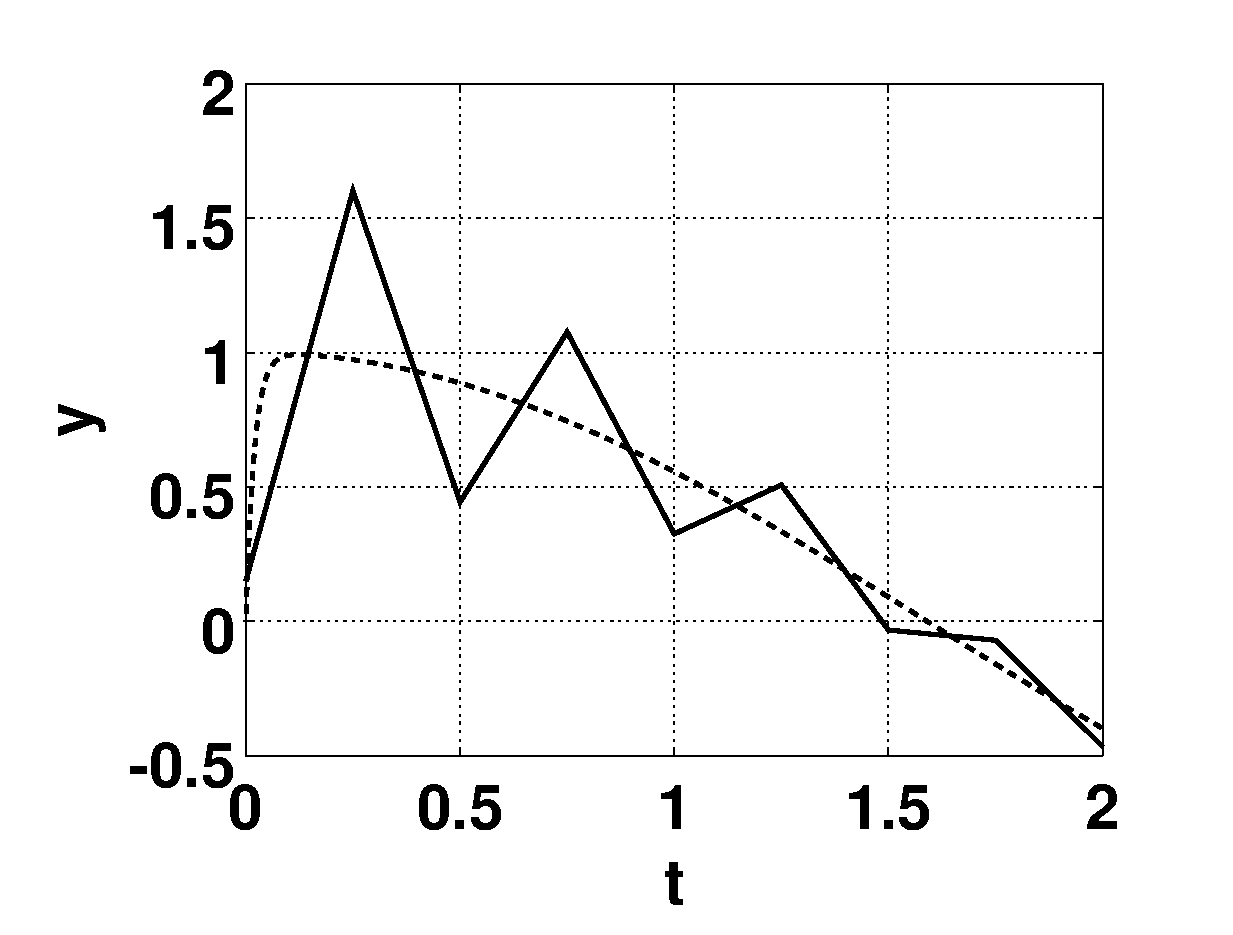
\includegraphics[width=6.5cm]{img/imp_mid.eps}
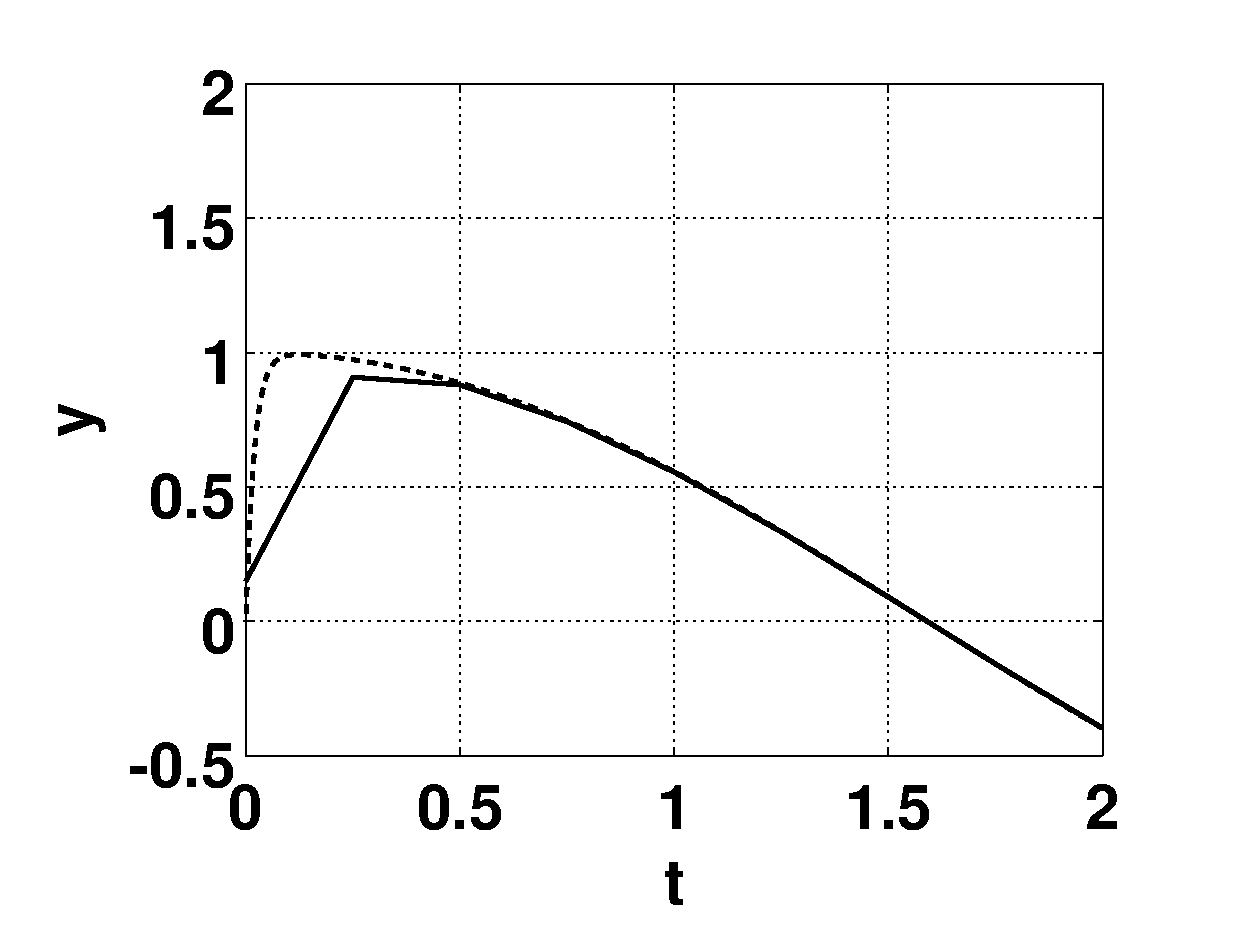
\includegraphics[width=6.5cm]{img/eul_imp.eps}
\caption{Solution of Curtis-Hirschfelder equation using implicit midpoint(left) and Euler implicit(right) methods. The former method is only \textit{A-stable} while the latter is also \textit{L-stable}. The dotted line represents in both cases the exact solution.}\label{fig:A_stability}
\end{figure}

\subsection{Stiff problems}
The concern about stability of a numerical solution is due to the resolution of \textit{stiff} problems. There is not a universally accepted definition of \textit{stiffness} of an ODE problem, but a possible tentative characterization is the following
\theoremstyle{definition}
\begin{definition}{}
A stable problem $\frac{\text{d}}{\text{d} t}y = f(t,y)$ is called \textit{stiff} when $\max_{i}\vert \lambda_i \vert$ is large, where $\lambda_i$ is an eigenvalue of $\frac{\partial f}{\partial y}$, with coefficients frozen at some $(t_0,y_0)$. $L:=\max_i\vert \Re(\lambda_i) \vert$ is sometimes called \textit{stiffness} index and gives an hint about the magnitude of the \textit{stiffness}, while usually the letter $\rho$ is usually used to refere to $\max_{i}\vert \lambda_i \vert$.
\end{definition}{}
For a numerical method to be stable $z=\Delta t \rho$ need to be included in its stability domain. Since $\rho$ could be even of the scale of $10^6$ for common problems, a particularly small time step must be chosen in order to not have a solution that literally explodes after few steps. The time step required is influenced by different parameters, firstly by the nature of the problem, but also by the stability domain of the scheme employed. If the stablity domain is restricted to a small portion of the complex plane  near the origin, a very fine time step is used, even if we are not interested in having a so detailed picture of the solution in the that time interval. This issue should be taken into account every time we have to chose an ODE solver: sometimes the benefits of using an easy-to-implement and fast method are vanished by the insanely high number of steps required to \enquote{calm down} the solution. 

\section{Implicit methods: Solving a linear system}
\subsection{Implicit methods properties}
For implicit method, to find the stages defined in Definition \ref{def:RK_def} a system of non-linear equations has to be solved in order to find the different $\text{K}_i$. For fully implicit methods the dimensions of the system is equal to the number of stages, while for some other methods part of the stages could be determined explicitely. Even worse, if we are the dealing with an \textit{n}-dimensional problem, the dimension grow to $\textit{n}\times \text{(number o implicit stages)}$. This makes implicit methods more costly to implement and to be solved and more subject to round-off errors.
In \cite{Hairer_1} some tricks to reduce this kind of errors and make the non-linear system easier to be solved iteratively are introduced: the authors also present good choices for the initial state and  stopping criterion of the iterative procedure. One of the advices we want to report is the drawback of fixed point procedure to solve a non-linear system. Given a system of equation equation $\textbf{x}=\textbf{G}(\textbf{x})$, similar to the one that we have to solve for the stages, and provided a reasonably good starting guess for the solution $\textbf{x}^0$, this procedure requires to compute $\textbf{x}^{k+1}=\textbf{G}(\textbf{x}^k)$ until the difference between two iterations satisfies the requested tolerance. To converge, we need to work with a contraction, i.e.
\begin{equation*}
\norm{\textbf{G}(\textbf{x})-\textbf{G}(\textbf{y})}\leq \nu \norm{\textbf{x}-\textbf{y}}, \qquad 	\nu<1.
\end{equation*} 
If we consider that 
\begin{equation*}
\textbf{G}(\textbf{x})=\textbf{G}(\textbf{y})+\textbf{G}'(\textbf{y})(\textbf{x}-\textbf{y})+\dots ,
\end{equation*}
and for the problem arising from implicit methods we have, if $\textbf{x}^0$ is close to the solution then
\begin{equation*}
\nu \sim \norm{\textbf{G}'(\textbf{y})}\sim C \Delta t \rho.
\end{equation*}
But for stiff problems we know that $\rho$ could be very large: this means that what we have gain by using an implicit method will be lost since a very fine time step is required for convergence.
A better alternative to solve kind of problems is the Netwon-Raphson method, which relies on the computation % TODO

All these complexities are the price for a usually large stability domain. This is the reason for which they are the standard for solving really \text{stiff} problems.
We must pay attention to not think that any time discrretization will give a stable numerical solution: while it is true that the stability region is bigger than the one of explicit methods, only a sub set of implicit methods are \textit{A-stable} (see Figure \ref{fig:implicit_not_A_stable}).

\begin{figure}
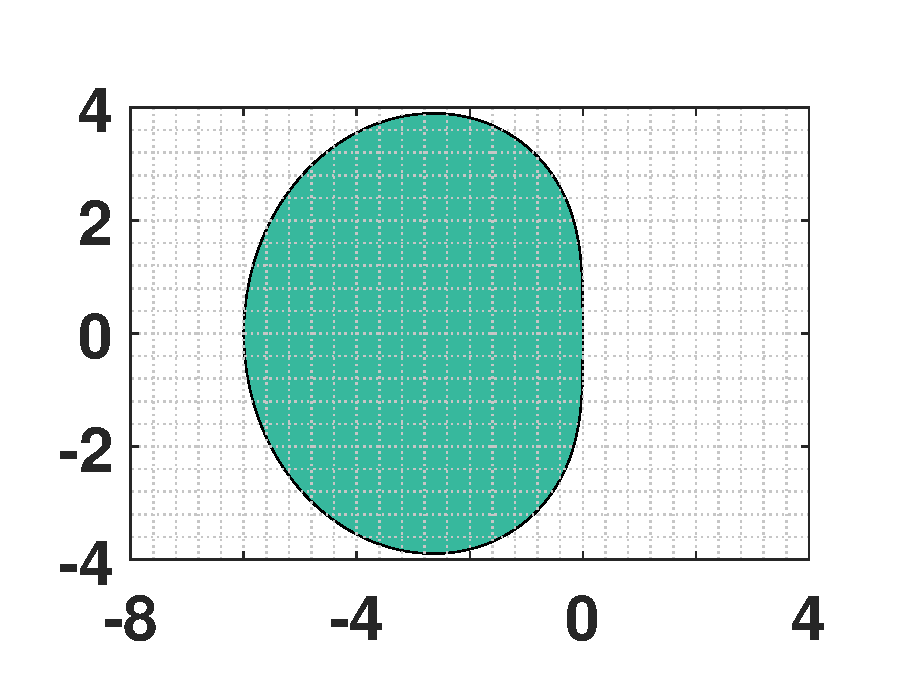
\includegraphics[width=4.15cm]{img/Hammer.eps}
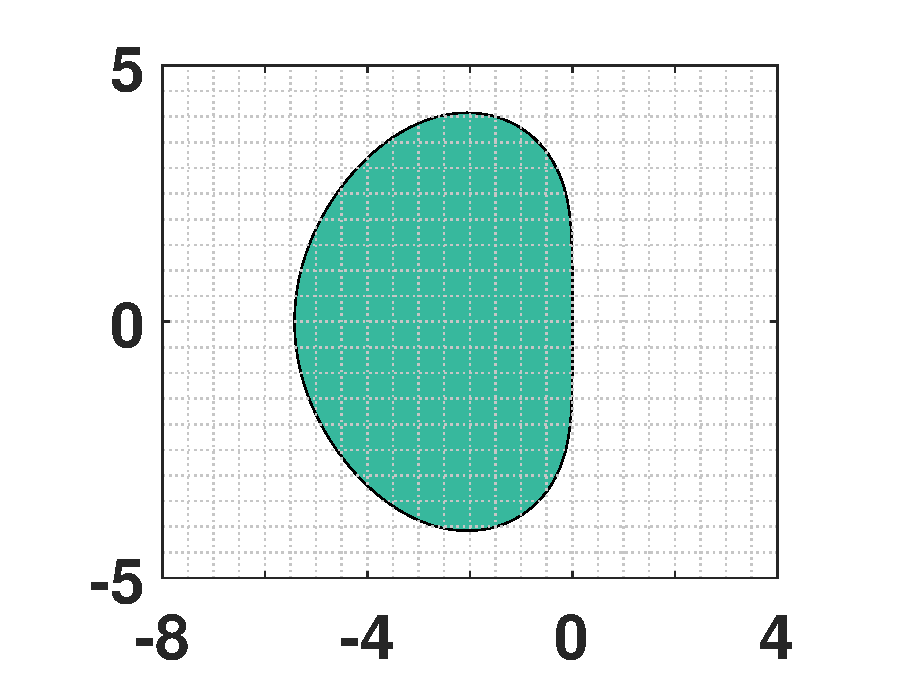
\includegraphics[width=4.15cm]{img/Lobatto_4.eps}
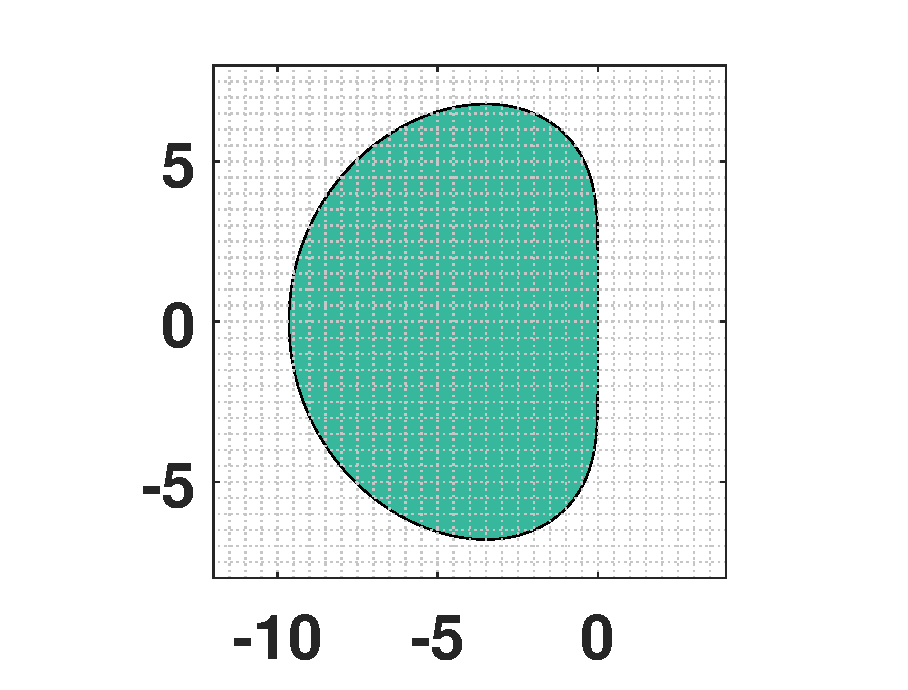
\includegraphics[width=4.15cm]{img/Lobatto_6.eps}
\caption{Stability regions of explicit Euler, implicit Euler and classical Runge-Kutta }
\label{fig:implicit_not_A_stable}
\end{figure}
\subsection{Strang splitting}
As we have seen in the previous section the non-linearity of the problem could cause some issues regarding instabilty and difficulties in the implementation. For particular class of operators the non-linearity could be killed by splitting the problem in the sum of linear operators, much easier to deal with. Here we will present a possible technique to address this splitting, with the approach \textit{divide et impera}.

Suppose we have the following differential equation that we want to integrate for a single time step $\Delta t$
\begin{equation}
\frac{\text{d}}{\text{d}t}y=f(y,t)=f_1(y,t)+f_2(y,t),\label{eqn:unsplit}
\end{equation}
and that
\begin{align*}
\frac{\text{d}}{\text{d} t}y &= f_1(y,t),\\
\frac{\text{d}}{\text{d} t}y &= f_2(y,t)w,
\end{align*}
happen to be easier problems than the original (no non-linearities, know exact solutions, \dots).
The idea for the construction of the new method is to solve first one of the two problems with a certain initial data
\begin{equation*}
\frac{\text{d}}{\text{d}t}y=f_1(y,t), \qquad y(0)=y_n.
\end{equation*}
This take us to $y^*=y_1(\Delta t;y_s)$, where $y_1$ represents the solution of the differential equation on vector field $f_1$. As next step, we start from $y^*$ and solve the second initial value problem
\begin{equation*}
\frac{\text{d}}{\text{d}t}y=f_2(y,t), \qquad y(0)=y^*.
\end{equation*}
on the same interval $\Delta t$ to obtain $y_{n+1}=y_2(\Delta t;y^*)$
It is possible to reinterpret this procedure in terms of \textit{flows}\cite{Hairer_1}
\theoremstyle{definition}
\begin{definition}{}
The \textit{flow} of a system $\frac{\text{d}}{\text{d} t}=f(y,t)$ is the mapping which, to any point $y_0$ in the phase space, associates the value $y(t)$ of the solution with initial value $y(0)=y_0$. This map, denoted by $\phi_t$, is thus defined by
\begin{equation*}
\phi_t(y_0)=y(t), \quad if \quad y(0)=y_0.
\end{equation*}
\end{definition}{}
Denoting the flow related to $f_1$ and $f_2$ as $\phi_{t,f_1}$ and $\phi_{t,f_2}$ respectively, what we have previously computed is $y_{n+1}=\phi_{\Delta t,f_2}(\phi_{\Delta t,f_1}(y_n))=(\phi_{\Delta t,f_2}\circ\phi_{\Delta t,f_1})(y_n)=\phi^{T\text{--}L}_{\Delta t, f}(y_n)$. This is an example of a \textit{splitting method}, the \textit{Lie-Trotter splitting}. Since the order of the operators is arbitrary, also $y_{n+1}=(\phi_{\Delta t,f_1}\circ\phi_{\Delta t,f_2})(y_n)=(\phi^{{T\text{--}L}}_{\Delta t, f})^*(y_n)$ would have been a viable choice (and we obtain the adjoint of the previous operator). By Taylor's expansion we can prove that
\begin{align*}
(\phi_{\Delta t,f_1}\circ\phi_{\Delta t,f_2})(y_0)&=\phi_{\Delta t,f}(y_0)+\mathcal{O}(h^2)\\
(\phi_{\Delta t,f_2}\circ\phi_{\Delta t,f_1})(y_0)&=\phi_{\Delta t,f}(y_0)+\mathcal{O}(h^2)
\end{align*}
and so both the methods gives only a $1^{st}$ order approximation of the solution to (\ref{eqn:unsplit})

\begin{figure}
\centering
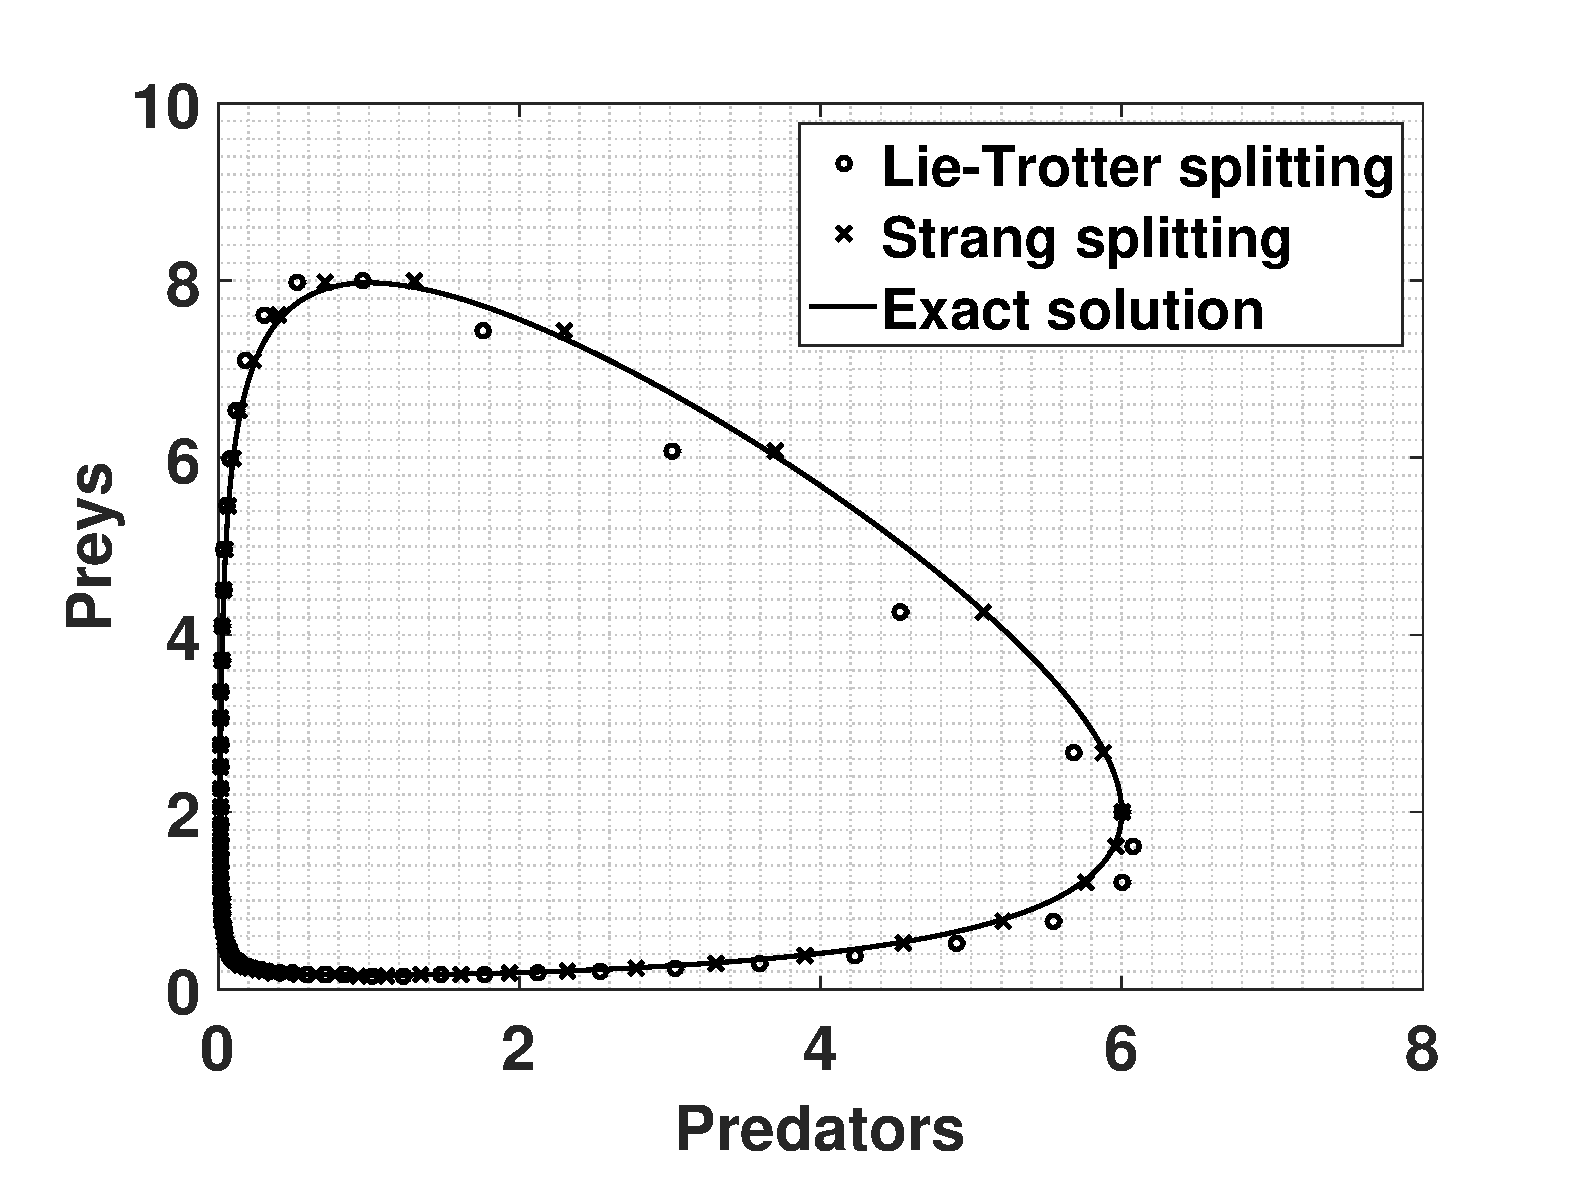
\includegraphics[width=7cm]{img/lotka_volterra.eps}
\caption{Solution of Lotka-Volterra equation \cite{Lotka}. Comparison between exact solution and different splitting techniques. }
\end{figure}
\section{Explicit methods: Stabilizing with stages}


\chapter{Setting of the problem}
\textbf{Cable equation}:
\begin{align*}
10^{-3}C_M\frac{\partial V}{\partial t}=&\frac{10^4}{2aR}\frac{\partial}{\partial x}\left(a^2\frac{\partial V}{\partial x}\right)\\
&-\bar{g}_\text{K}n^4(V-V_\text{K})- \bar{g}_\text{Na}m^3h(V-V_\text{Na})-\bar{g}_\text{L}(V-V_\text{L})\\
&-\frac{10^2g_{syn}y}{2\pi a}\delta_{syn}(x)(V-V_{syn}),
\end{align*}
Boundary conditions:
\begin{itemize}
\item Branching node
\begin{equation*}
\left( a^2\frac{\partial V}{\partial x}\right)\bigg|_{x=x_b}^A=\left( a^2\frac{\partial V}{\partial x}\right)\bigg|_{x=x_b}^{B_1}+\left( a^2\frac{\partial V}{\partial x}\right)\bigg|_{x=x_b}^{B_2}
\end{equation*}
\item Terminal nodes
\begin{equation*}
\frac{\partial V}{\partial x}=0
\end{equation*}
\end{itemize}
Initial condition:
\begin{equation*}
V\bigg|_{t=0}=V_0
\end{equation*}
\textbf{Gate states}:
\begin{align*}
\frac{dn}{dt}&=\alpha_n(1-n)-\beta_nn\\
\frac{dm}{dt}&=\alpha_m(1-m)-\beta_mm\\
\frac{dh}{dt}&=\alpha_h(1-h)-\beta_hh
\end{align*}
Initial conditions
\begin{align*}
n_0&=\frac{\alpha_n\vert_{V=0}}{\alpha_n\vert_{V=0}+\beta_n\vert_{V=0}}\\
m_0&=\frac{\alpha_m\vert_{V=0}}{\alpha_m\vert_{V=0}+\beta_m\vert_{V=0}}\\
h_0&=\frac{\alpha_h\vert_{V=0}}{\alpha_h\vert_{V=0}+\beta_h\vert_{V=0}}
\end{align*}

%----------------------------------------------------------------------
%       BIBLIOGRAPHY
%----------------------------------------------------------------------

\renewcommand\bibname{References}
\printbibliography
\addcontentsline{toc}{chapter}{References}

\end{document}
